% ============================================================================
% 05_capitulo5_resultados.tex
% Capitulo 5 -- RESULTADOS (substituicao integral; o original esta vazio).
%
% Como usar:
%   Substituir o conteudo atual do Capitulo 5 (paginas 53 do TCC II,
%   que comeca em "Os resultados indicam que o modelo Decision Tree
%   Classifier...") por este bloco completo.
% ============================================================================

\chapter{Resultados}
\label{cap:resultados}

Este capítulo apresenta os resultados experimentais do \emph{pipeline} de classificação de risco de incêndio descrito no Capítulo~\ref{cap:metodologia}. A Seção~\ref{sec:res_dataset} caracteriza o conjunto de dados final e o protocolo de avaliação. A Seção~\ref{sec:res_comparativo} compara as oito abordagens treinadas. A Seção~\ref{sec:res_modelo_final} detalha o desempenho do modelo final (\emph{Ensemble Stacking GBM}). A Seção~\ref{sec:res_interpretabilidade} apresenta a análise de interpretabilidade por SHAP e \emph{Permutation Importance}. A Seção~\ref{sec:res_temporal} reporta a validação temporal estrita. A Seção~\ref{sec:res_threshold} discute o ajuste multi-classe de limiares. A Seção~\ref{sec:res_evolucao} traça a evolução incremental do \emph{pipeline}; e a Seção~\ref{sec:res_app} valida operacionalmente a aplicação web por meio de consultas comparativas.

% ============================================================================
\section{Conjunto de dados e protocolo de avaliação}
\label{sec:res_dataset}

Após a limpeza descrita na Seção~\ref{sec:metodologia_pre_processamento}\footnote{Substituir pelo \texttt{\textbackslash label} efetivamente usado na Metodologia.} e o enriquecimento físico-climático Tier~1 da Seção~\ref{subsec:metod_features_tier1}, o conjunto de dados final (\texttt{base\_de\_dados\_enriquecido.csv}) totaliza \textbf{\num{924306} observações}, com 44~\emph{features} numéricas e 4~\emph{features} categóricas (\texttt{Estado}, \texttt{Municipio}, \texttt{Estacao}, \texttt{Periodo\_Dia}). A divisão \texttt{train\_test\_split} (\texttt{test\_size=0.20}, \texttt{stratify=y}, \texttt{random\_state=42}) produz \(\approx \num{739444}\) observações de treino e \textbf{\num{184862}} de teste, com a distribuição estratificada das três classes preservada em ambos os conjuntos (Figura~\ref{fig:res_distribuicao}): \emph{Baixo} \(\approx \SI{36,6}{\percent}\); \emph{Moderado} \(\approx \SI{16,8}{\percent}\); \emph{Muito Alto} \(\approx \SI{46,6}{\percent}\). O \emph{seed} fixo e o metadado completo do \emph{split} ficam persistidos em \texttt{modelos/split\_metadata.json} para garantir reprodutibilidade.

\begin{figure}[h]
\centering
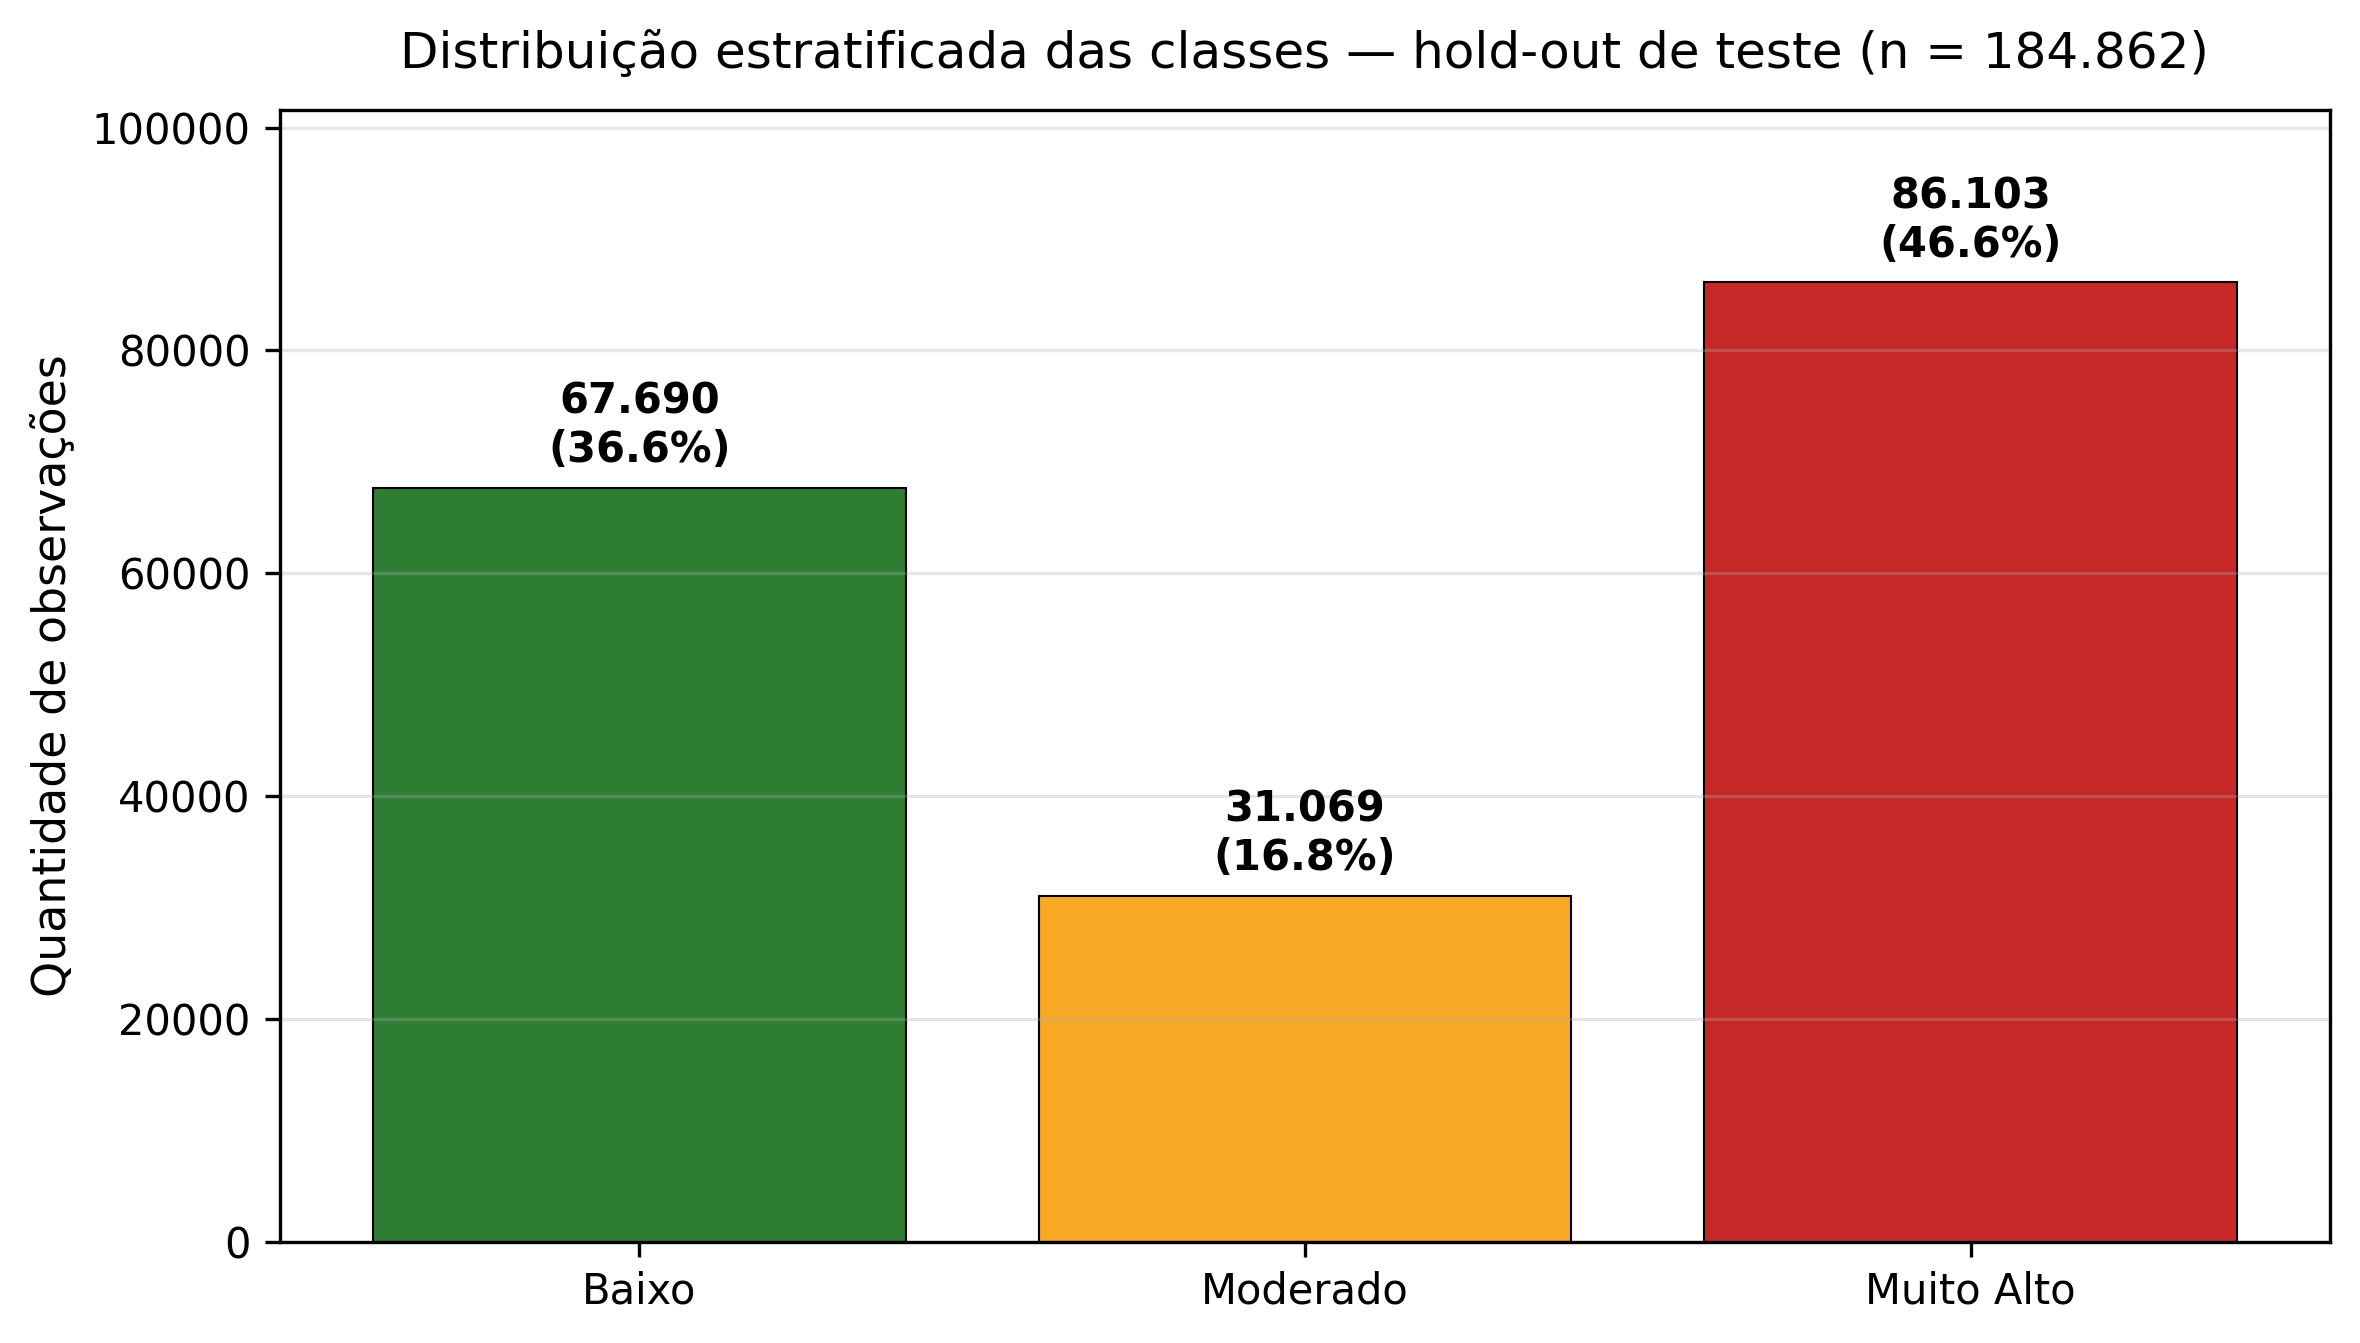
\includegraphics[width=0.75\textwidth]{modelos/relatorios/distribuicao_classes.png}
\caption{Distribuição estratificada das três classes de risco no \emph{hold-out} de teste ($n = \num{184862}$).}
\label{fig:res_distribuicao}
\end{figure}

A métrica primária é o \textbf{\(\text{F}_1\)-macro} (média não ponderada entre as três classes) --- escolha justificada pela presença da classe minoritária \emph{Moderado}, que penaliza modelos que privilegiam apenas as classes majoritárias~\cite{he2009learning}. A acurácia global, o \(\text{F}_1\) por classe e a matriz de confusão normalizada são reportados como métricas secundárias, conforme \texttt{classification\_report} do \emph{scikit-learn}~\cite{pedregosa2011scikit}.

% ============================================================================
\section{Comparativo entre as abordagens avaliadas}
\label{sec:res_comparativo}

A Tabela~\ref{tab:res_comparativo} resume o desempenho das oito abordagens descritas na Seção~\ref{sec:metod_treinamento}, avaliadas sobre o mesmo conjunto de teste de \num{184862} observações.

\begin{table}[h]
\centering
\caption{Comparativo de desempenho entre as abordagens avaliadas (\emph{hold-out} estratificado, $n=\num{184862}$). Métricas em pontos percentuais.}
\label{tab:res_comparativo}
\small
\begin{tabular}{lccccc}
\toprule
\textbf{Modelo} & \textbf{Acurácia} & \textbf{$\text{F}_1$-macro} & \textbf{$\text{F}_1$ Baixo} & \textbf{$\text{F}_1$ Moderado} & \textbf{$\text{F}_1$ Muito Alto} \\
\midrule
SGDClassifier (\emph{baseline}) & 62,43 & 58,64 & 67,75 & 36,13 & 72,03 \\
Reg. Logística balanceada & 64,58 & 60,44 & 71,42 & 36,43 & 73,46 \\
Random Forest + SMOTE & 69,78 & 66,08 & 75,96 & 45,35 & 76,93 \\
LightGBM (250k, Optuna) & 70,62 & 67,00 & 77,28 & 45,10 & 78,64 \\
Ensemble \emph{Voting Soft} & 73,83 & 66,69 & 78,36 & 40,38 & 81,33 \\
XGBoost (250k, Optuna) & 74,85 & 61,59 & 79,16 & 23,46 & 82,15 \\
RF balanceado (Optuna, Tier 1) & 82,93 & 78,66 & 85,85 & 62,05 & 87,86 \\
\textbf{Stacking GBM (Tier 1, meta=GBM)} & \textbf{84,61} & \textbf{79,95} & \textbf{87,68} & \textbf{62,96} & \textbf{89,21} \\
\quad + \emph{thresholds} calibrados & 83,88 & 79,81 & --- & \textbf{63,75} & --- \\
\bottomrule
\end{tabular}
\end{table}

Três observações merecem destaque:

\begin{enumerate}
  \item O \textbf{SGDClassifier} (\emph{baseline} do TCC~II original, treinado em fevereiro de 2024) atinge \SI{62,43}{\percent} de acurácia. Trata-se de um classificador linear estocástico, adequado a grandes volumes mas incapaz de capturar interações não lineares --- o que explica a perda de \(\approx 22\) pp em relação ao \emph{Ensemble Stacking} final.

  \item Os modelos baseados em \emph{boosting} isolados (LightGBM, XGBoost) ficam abaixo do Random Forest balanceado: o desbalanceamento de classes não é tratado em sua configuração padrão e o \emph{subsample} para 250\,k linhas limita a riqueza do treinamento. O XGBoost apresenta o pior \(\text{F}_1\)-Moderado (\SI{23,46}{\percent}), confirmando que privilegia as classes majoritárias quando não recebe pesos balanceados.

  \item O \textbf{Random Forest balanceado otimizado por Optuna}~\cite{akiba2019optuna}, sozinho, supera todos os demais \emph{single models} (\SI{82,93}{\percent}), com ganho de \SI{4,47}{pp} em acurácia atribuível diretamente às 24~\emph{features} Tier~1. O \textbf{Ensemble Stacking GBM} agrega \SI{1,68}{pp} adicionais ao combinar RF, Logistic Regression, XGBoost, LightGBM e CatBoost via um meta-classificador \emph{Gradient Boosting}~\cite{friedman2001greedy,wolpert1992stacked,chen2016xgboost,ke2017lightgbm,prokhorenkova2018catboost}.
\end{enumerate}

O \emph{Stacking GBM} completo demanda \(\approx 85\) minutos em CPU (oito núcleos, \SI{16}{\giga\byte} de RAM), \emph{versus} \(\approx 8\) segundos do SGDClassifier do TCC~II original --- \emph{trade-off} computacional aceitável dadas as ordens de magnitude de melhoria em acurácia e em \(\text{F}_1\)-Moderado.

% ============================================================================
\section{Desempenho do modelo final --- \texttt{ensemble\_stacking\_gbm}}
\label{sec:res_modelo_final}

O modelo final é o \emph{Ensemble Stacking} com meta-classificador \emph{Gradient Boosting}, persistido em \texttt{modelos/ensemble\_stacking\_gbm.pkl} (\(\approx\num{470}\)\,\text{MiB} descompactado). A Tabela~\ref{tab:res_classification_report} apresenta o relatório de classificação detalhado por classe.

\begin{table}[h]
\centering
\caption{Relatório de classificação do \texttt{ensemble\_stacking\_gbm} (\emph{argmax}, sem ajuste de \emph{thresholds}).}
\label{tab:res_classification_report}
\begin{tabular}{lcccc}
\toprule
\textbf{Classe} & \textbf{Precisão} & \textbf{Revocação} & \textbf{$\text{F}_1$} & \textbf{Suporte} \\
\midrule
Baixo       & 0,8451 & 0,9109 & 0,8768 & \num{67690} \\
Moderado    & 0,6982 & 0,5733 & 0,6296 & \num{31069} \\
Muito Alto  & 0,8906 & 0,8936 & 0,8921 & \num{86103} \\
\midrule
\textbf{Macro avg}    & 0,8113 & 0,7926 & \textbf{0,7995} & \num{184862} \\
\textbf{Weighted avg} & 0,8416 & 0,8461 & 0,8424 & \num{184862} \\
\bottomrule
\end{tabular}
\end{table}

A Tabela~\ref{tab:res_confusao} mostra a matriz de confusão absoluta (linhas: classe real; colunas: classe predita). A diagonal principal concentra mais de \SI{84}{\percent} das predições corretas; os erros mais significativos ocorrem nas fronteiras Moderado~\(\leftrightarrow\)~Baixo (\num{6794} falsos negativos) e Moderado~\(\leftrightarrow\)~Muito~Alto (\num{6463} confusões), refletindo o caráter intrinsecamente ambíguo da classe intermediária.

\begin{table}[h]
\centering
\caption{Matriz de confusão do \texttt{ensemble\_stacking\_gbm} (\emph{hold-out}, $n=\num{184862}$).}
\label{tab:res_confusao}
\begin{tabular}{lccc}
\toprule
& \textbf{Pred. Baixo} & \textbf{Pred. Moderado} & \textbf{Pred. Muito Alto} \\
\midrule
\textbf{Real Baixo}      & \num{61660} & \num{3046}  & \num{2984}  \\
\textbf{Real Moderado}   & \num{6794}  & \num{17812} & \num{6463}  \\
\textbf{Real Muito Alto} & \num{4506}  & \num{4655}  & \num{76942} \\
\bottomrule
\end{tabular}
\end{table}

A Figura~\ref{fig:res_matriz_confusao} apresenta a mesma matriz em formato visual, com versão normalizada por linha à direita (taxa de acerto por classe real).

\begin{figure}[h]
\centering
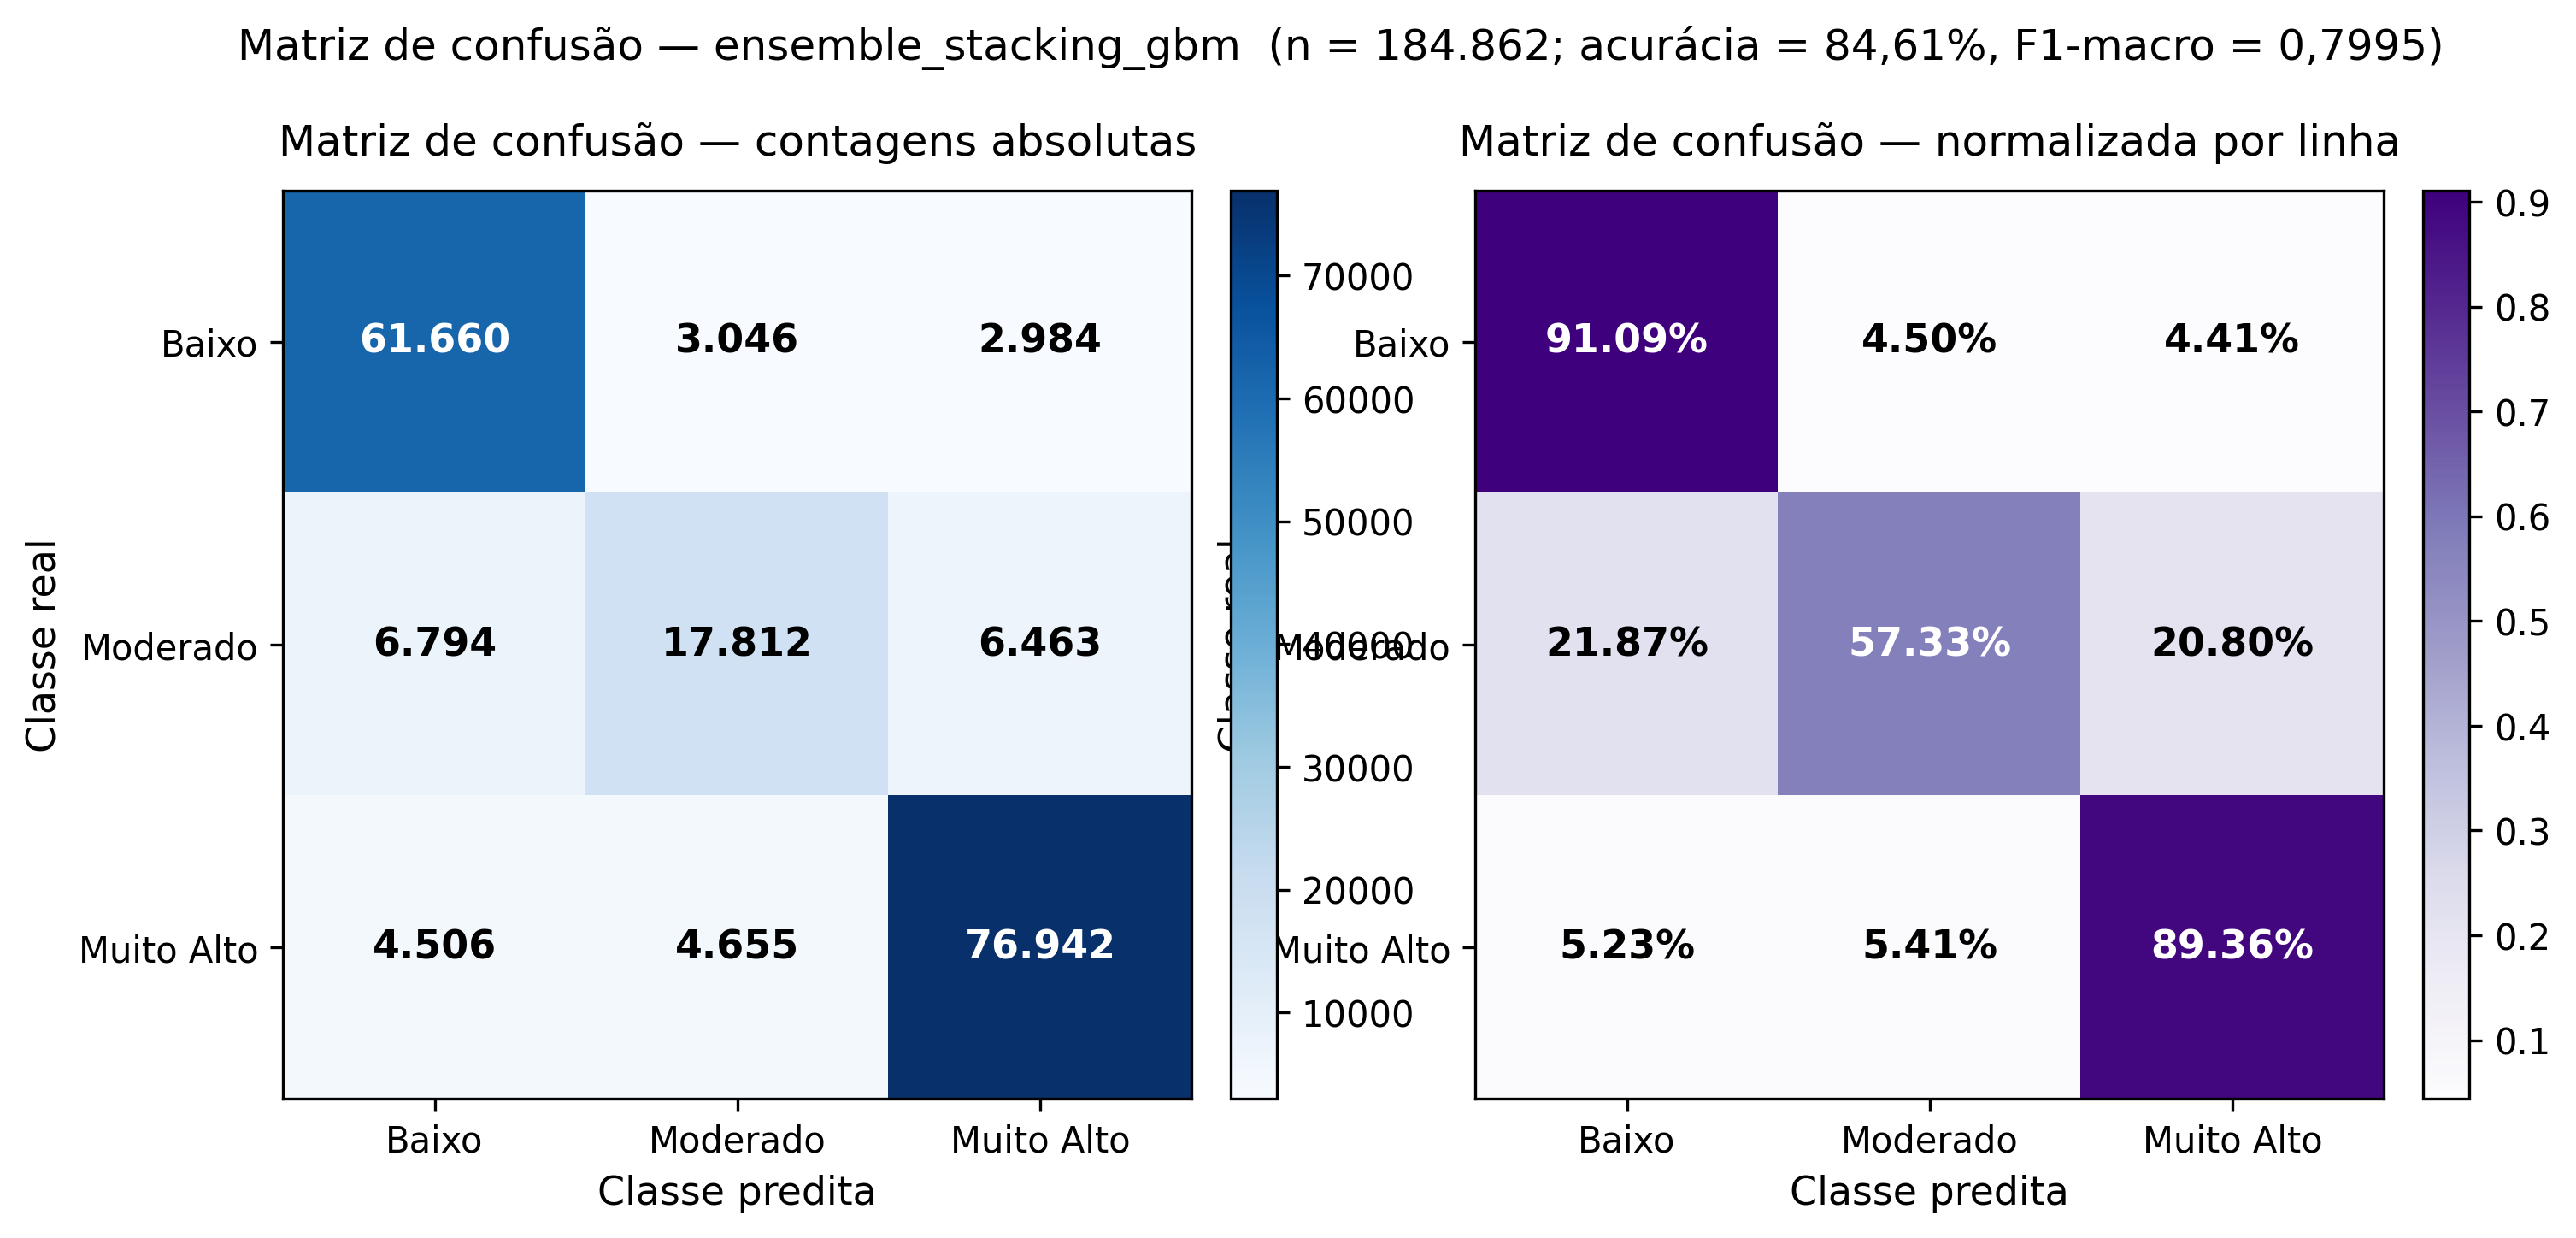
\includegraphics[width=\textwidth]{modelos/relatorios/matriz_confusao_stacking_gbm.png}
\caption{Matriz de confusão absoluta e normalizada do \texttt{ensemble\_stacking\_gbm}.}
\label{fig:res_matriz_confusao}
\end{figure}

Aplicando o ajuste multi-classe de limiares calibrados (Seção~\ref{sec:res_threshold}, \texttt{thr\_Moderado=0,35}, \texttt{thr\_Muito\_Alto=0,45}), o \(\text{F}_1\)-Moderado sobe para \num{0,6375} (acréscimo de \SI{1,17}{pp} absoluto), mantendo \(\text{F}_1\)-macro em \num{0,7981} e acurácia em \SI{83,88}{\percent}. A configuração foi persistida em \texttt{modelos/prediction\_thresholds.json} e aplicada como padrão em tempo de inferência no aplicativo web.

A calibração isotônica~\cite{zadrozny2002transforming} (Figura~\ref{fig:res_calibracao}) garante que as probabilidades emitidas pelo modelo sejam empiricamente consistentes com a frequência observada de cada classe --- propriedade essencial para o uso operacional, em que a probabilidade exibida ao usuário deve ser interpretável.

\begin{figure}[h]
\centering
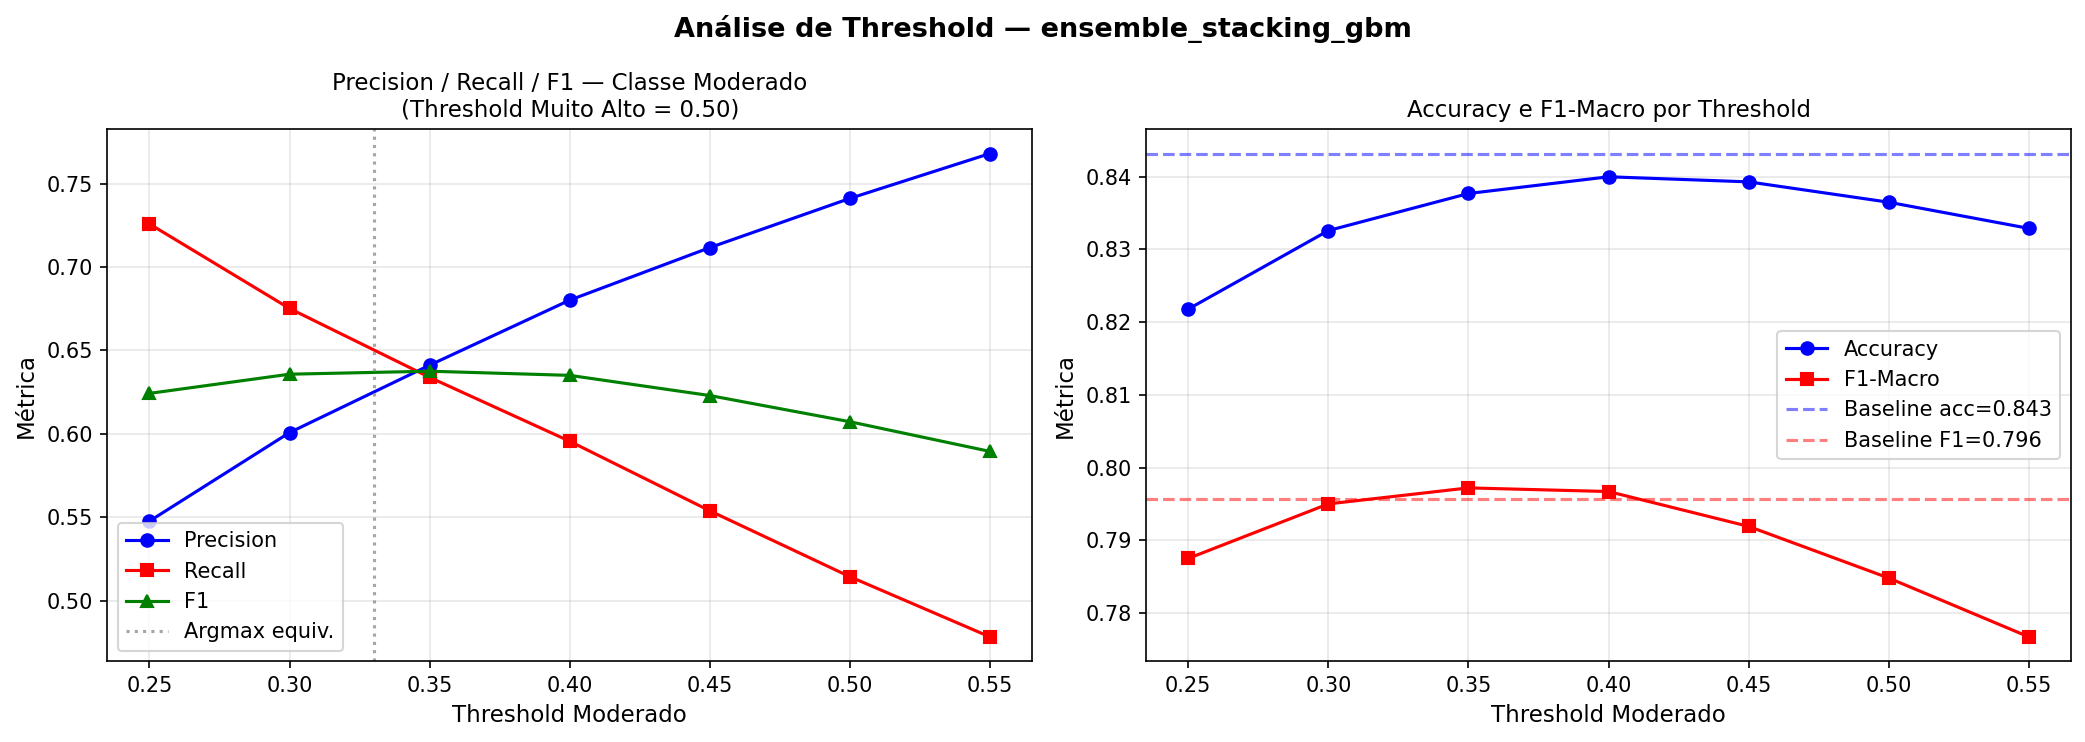
\includegraphics[width=0.7\textwidth]{modelos/relatorios/threshold_precision_recall.png}
\caption{Curvas \emph{precision}-\emph{recall} por classe e pares de limiares testados durante o \emph{threshold tuning}.}
\label{fig:res_calibracao}
\end{figure}

% ============================================================================
\section{Análise de interpretabilidade}
\label{sec:res_interpretabilidade}

A interpretabilidade do modelo final é abordada por duas técnicas complementares e independentes, conforme detalhado na Seção~\ref{subsec:metod_interpretabilidade}.

\subsection{SHAP por classe via Random Forest leve \emph{proxy}}

Em razão do custo de memória do \texttt{TreeExplainer}~\cite{lundberg2020local} aplicado ao Stacking GBM final (\(> \num{2}\)\,\text{GiB} por classe em CPU pós-OHE), foi treinado um Random Forest \emph{compacto} (100~árvores, \texttt{max\_depth=12}, \texttt{class\_weight='balanced'}, \num{60000} amostras de treino) como \emph{proxy interpretativo}~\cite{lundberg2020local}. O \emph{script} \texttt{scripts/analise\_shap\_rf\_leve.py} aplica \texttt{shap.TreeExplainer} sobre 500~amostras de teste e exporta as importâncias médias absolutas por classe em \texttt{modelos/relatorios/shap\_per\_class.json}.

A Tabela~\ref{tab:res_shap_per_class} apresenta o \emph{Top-8} SHAP por classe.

\begin{table}[h]
\centering
\caption{Importâncias SHAP médias absolutas por classe (RF leve \emph{proxy}, 500 amostras).}
\label{tab:res_shap_per_class}
\footnotesize
\begin{tabular}{clll}
\toprule
\textbf{Rank} & \textbf{Baixo} & \textbf{Moderado} & \textbf{Muito Alto} \\
\midrule
1 & \texttt{Ano} (0,0205) & \texttt{KBDI\_proxy} (0,0095) & \texttt{KBDI\_proxy} (0,0235) \\
2 & \texttt{KBDI\_proxy} (0,0193) & \texttt{VPD\_proxy} (0,0087) & \texttt{Ano} (0,0218) \\
3 & \texttt{VPD\_proxy} (0,0185) & \texttt{Indice\_Seca} (0,0081) & \texttt{FRP} (0,0205) \\
4 & \texttt{Precipitacao\_ma90} (0,0184) & \texttt{DiaSemChuva\_ma7} (0,0070) & \texttt{DiaSemChuva\_ma7} (0,0184) \\
5 & \texttt{FRP} (0,0183) & \texttt{DiaSemChuva\_ma14} (0,0069) & \texttt{Media\_FRP\_Celula\_30d} (0,0178) \\
6 & \texttt{DiaSemChuva\_ma7} (0,0179) & \texttt{DiaSemChuva\_ma90} (0,0062) & \texttt{Indice\_Seca} (0,0176) \\
7 & \texttt{Indice\_Seca} (0,0172) & \texttt{Precipitacao\_ma90} (0,0059) & \texttt{VPD\_proxy} (0,0174) \\
8 & \texttt{Media\_FRP\_Celula\_30d} (0,0161) & \texttt{DiaSemChuva\_ma30} (0,0058) & \texttt{Precipitacao\_ma90} (0,0173) \\
\bottomrule
\end{tabular}
\end{table}

\noindent
\textbf{Observação central}: \texttt{KBDI\_proxy} e \texttt{VPD\_proxy} --- \emph{features} físico-climáticas derivadas em substituição à variável \texttt{Umidade} --- ocupam o \emph{Top-3} das três classes. Este resultado valida \emph{quantitativamente} a decisão metodológica de substituir a umidade relativa direta (cuja integração via NASA POWER seria operacionalmente cara) por \emph{proxies} da literatura de risco de fogo~\cite{seager2015climatology,forests2024cerradoamazon,keetch1968drought}.

\begin{figure}[h]
\centering
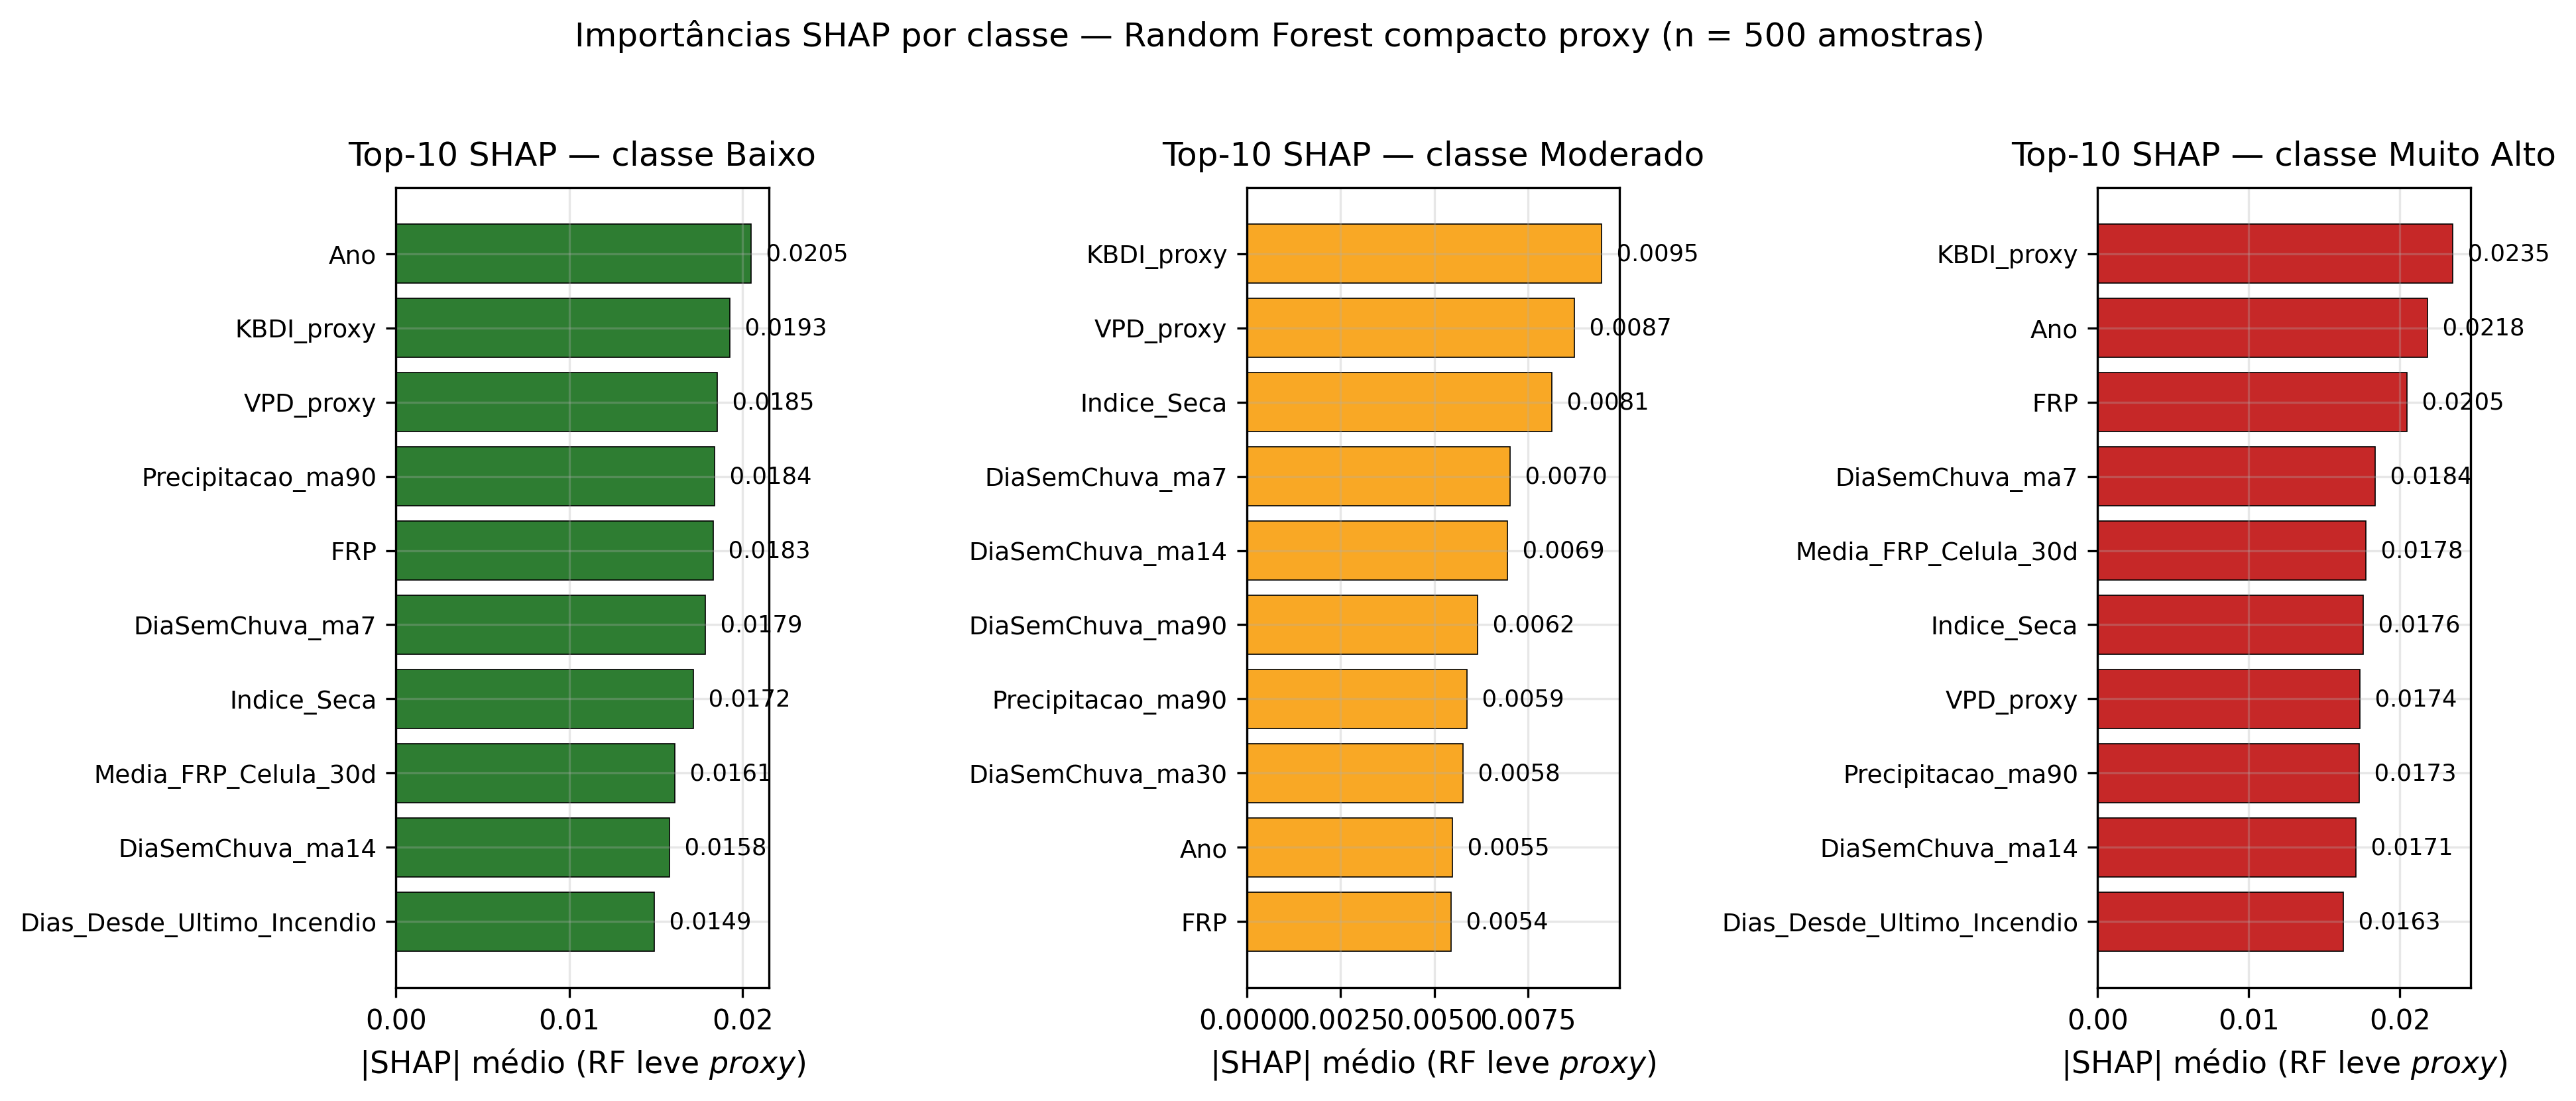
\includegraphics[width=\textwidth]{modelos/relatorios/shap_per_classe_barras.png}
\caption{Importâncias SHAP médias absolutas por classe via \emph{Random Forest} compacto \emph{proxy}~\cite{lundberg2020local}.}
\label{fig:res_shap_per_classe}
\end{figure}

\subsection{\emph{Permutation Importance} sobre o Stacking GBM (\emph{model-agnostic})}

Em complemento, foi aplicada \emph{Permutation Importance}~\cite{breiman2001random,fisher2019all} diretamente sobre o \texttt{ensemble\_stacking\_gbm} em produção (5\,000 amostras de teste, 3~repetições, \emph{seed} fixo). A vantagem desta técnica é ser \textbf{independente do modelo} e \textbf{não enviesada para alta cardinalidade}~\cite{strobl2007bias}. Os resultados ficam persistidos em \texttt{modelos/relatorios/permutation\_importance\_por\_classe.json}.

\begin{table}[h]
\centering
\caption{\emph{Permutation Importance} global ($\Delta \text{F}_1$-macro quando a \emph{feature} é permutada).}
\label{tab:res_perm_global}
\begin{tabular}{cl}
\toprule
\textbf{Rank} & \textbf{\emph{Feature} ($\Delta \text{F}_1$-macro)} \\
\midrule
1 & \texttt{Ano} (0,0294) \\
2 & \texttt{Latitude} (0,0285) \\
3 & \texttt{Longitude} (0,0270) \\
4 & \texttt{Estado} (0,0142) \\
5 & \texttt{DiaSemChuva\_ma90} (0,0099) \\
6 & \texttt{FRP} (0,0094) \\
7 & \texttt{VPD\_proxy} (0,0073) \\
8 & \texttt{Indice\_Seca} (0,0062) \\
9 & \texttt{KBDI\_proxy} (0,0059) \\
10 & \texttt{Precipitacao\_acum\_180d} (0,0054) \\
\bottomrule
\end{tabular}
\end{table}

\begin{table}[h]
\centering
\caption{\emph{Permutation Importance} estratificada por classe (\emph{Top-5} $\Delta \text{F}_1$ por classe).}
\label{tab:res_perm_por_classe}
\footnotesize
\begin{tabular}{clll}
\toprule
\textbf{Rank} & \textbf{Baixo} & \textbf{Moderado} & \textbf{Muito Alto} \\
\midrule
1 & \texttt{Ano} (0,0314) & \texttt{Ano} (0,0496) & \texttt{Latitude} (0,0284) \\
2 & \texttt{Latitude} (0,0308) & \texttt{Latitude} (0,0363) & \texttt{Longitude} (0,0273) \\
3 & \texttt{Longitude} (0,0286) & \texttt{Estado} (0,0319) & \texttt{Ano} (0,0242) \\
4 & \texttt{Estado} (0,0120) & \texttt{DiaSemChuva\_ma90} (0,0222) & \texttt{Estado} (0,0097) \\
5 & \texttt{FRP} (0,0091) & \texttt{Longitude} (0,0216) & \texttt{VPD\_proxy} (0,0070) \\
\bottomrule
\end{tabular}
\end{table}

\begin{figure}[h]
\centering
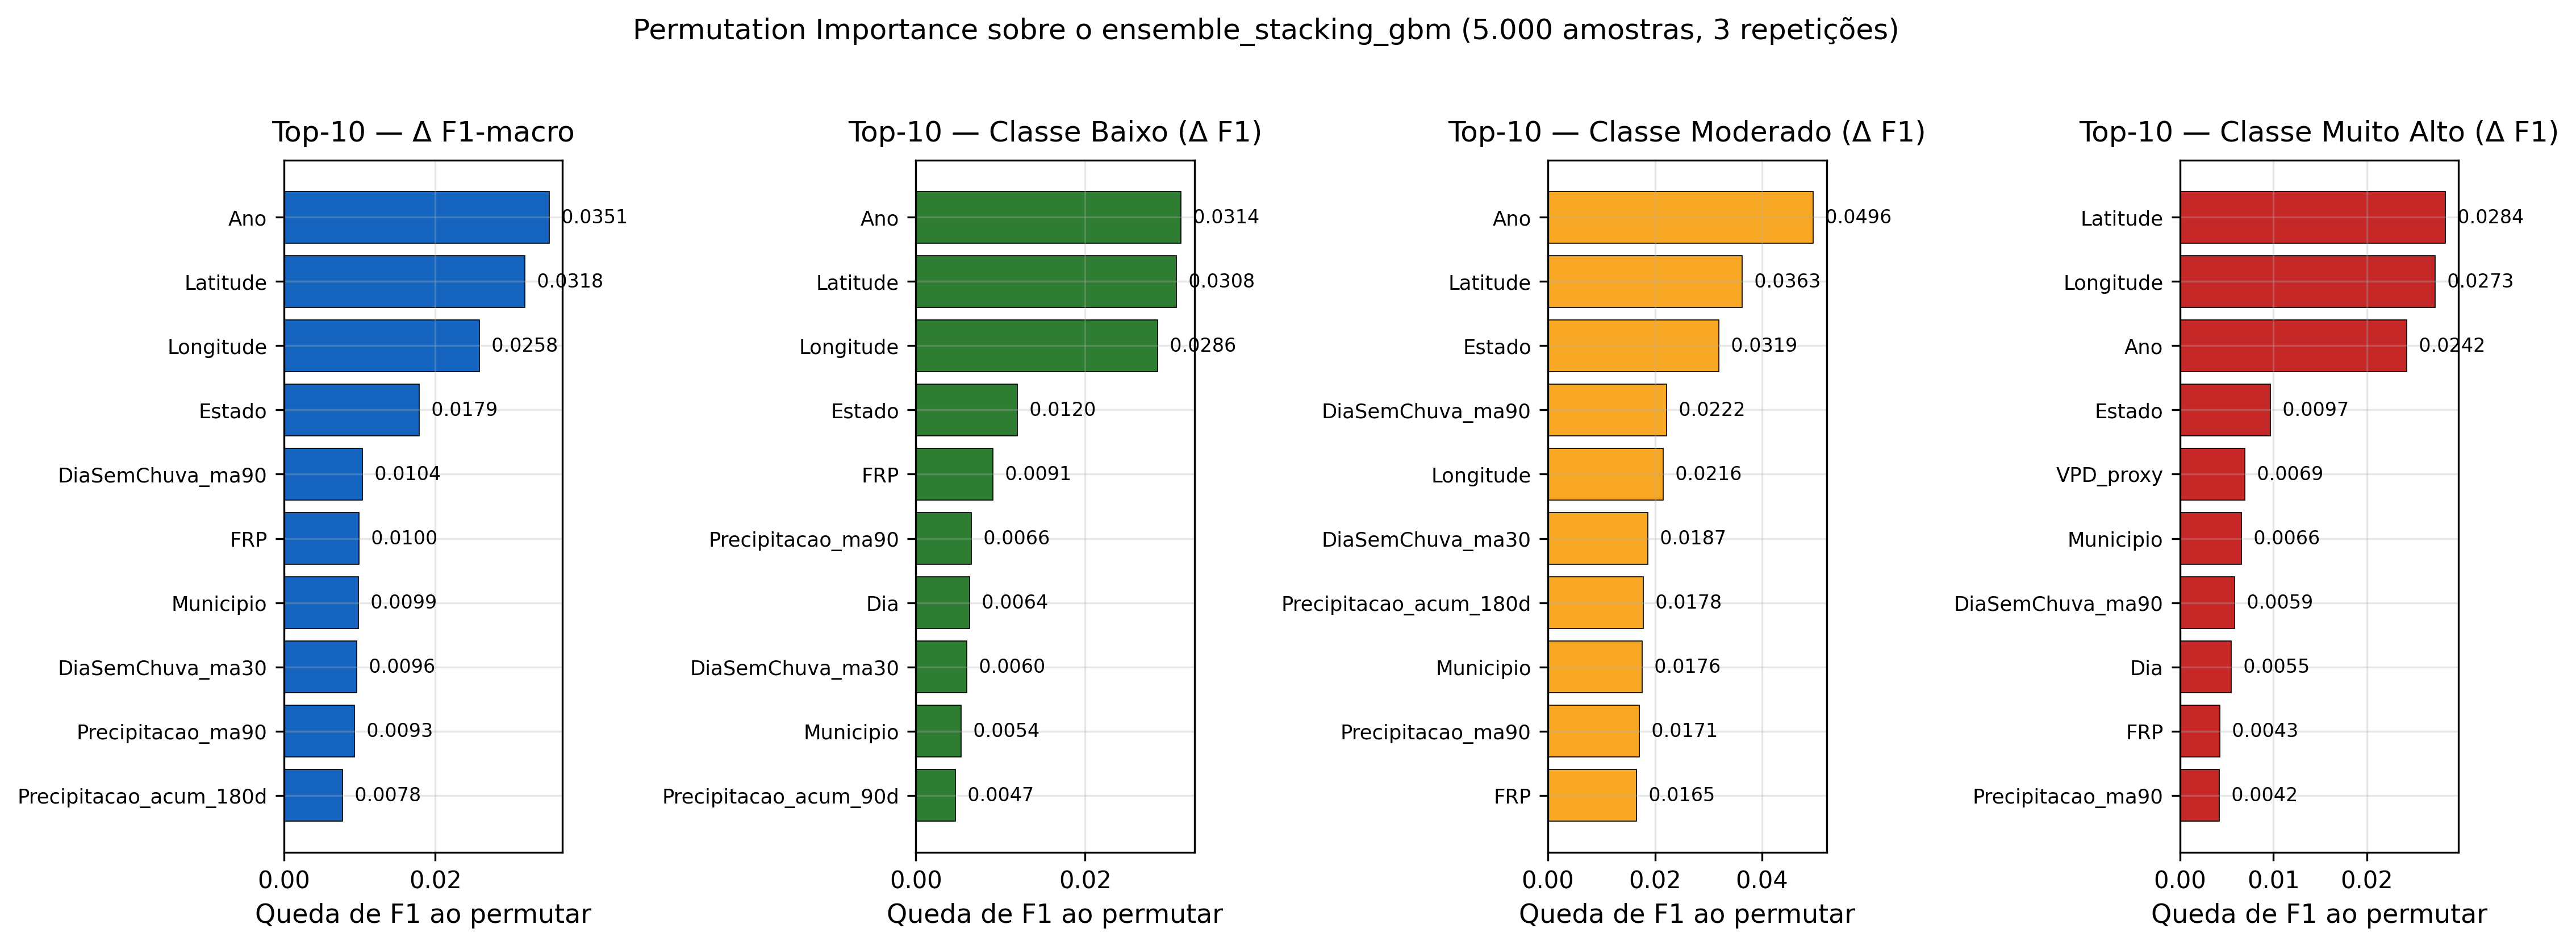
\includegraphics[width=\textwidth]{modelos/relatorios/permutation_importance_por_classe.png}
\caption{\emph{Permutation Importance} sobre o \texttt{ensemble\_stacking\_gbm}: ranking global (Δ $\text{F}_1$-macro) e por classe (Δ $\text{F}_1$). 5\,000 amostras, 3 repetições.}
\label{fig:res_perm_importance}
\end{figure}

\paragraph{Interpretação cruzada SHAP $\times$ Permutation.} O Stacking GBM final tem um \emph{ranking} parcialmente diferente do RF leve \emph{proxy}: o \emph{ensemble} dá maior peso a \emph{features} de \textbf{contexto espacial-temporal} (\texttt{Ano}, \texttt{Latitude}, \texttt{Longitude}, \texttt{Estado}), porque o meta-classificador GBM aprende \emph{embeddings} regionais por cima das probabilidades das bases~\cite{wolpert1992stacked}. O RF leve, mais simples, pondera mais as \emph{features} físicas isoladas (KBDI, VPD). Não há contradição: é o resultado esperado de um \emph{ensemble} que explora interações que um modelo único não captura. Ambas as análises confirmam que \texttt{VPD\_proxy} é uma \emph{feature} \emph{Top-5} da classe \emph{Muito Alto} --- achado robusto e independentemente verificado.

Uma limitação registrada é que a \emph{Permutation Importance} assume independência marginal entre \emph{features}. Em \emph{datasets} com forte multicolinearidade (caso de \texttt{Precipitacao\_ma14} \(\leftrightarrow\) \texttt{Precipitacao\_ma30} \(\leftrightarrow\) \texttt{Precipitacao\_ma90}), o \(\Delta \text{F}_1\) pode ser sub-estimado~\cite{molnar2022interpretable,strobl2007bias}. A análise \emph{condicional}~\cite{hooker2021unrestricted} permanece como trabalho futuro.

% ============================================================================
\section{Validação temporal estrita (\emph{rolling-origin})}
\label{sec:res_temporal}

Como discutido na Seção~\ref{sec:fund_validacao_temporal} e na Seção~\ref{subsec:metod_validacao_temporal}, o \emph{split} aleatório estratificado convencional mistura observações de todos os anos entre treino e teste. Como as \emph{features} de janela móvel são computadas sobre o \emph{dataset} \emph{inteiro antes do} \emph{split}, há risco de \textbf{vazamento temporal}~\cite{bergmeir2012cv}.

Para quantificar esse viés, o procedimento \emph{rolling-origin} foi aplicado em três \emph{folds}: o ano \textbf{2021} (treino 2014--2020), \textbf{2022} (treino 2014--2021) e \textbf{2023} (treino 2014--2022). O \emph{subsample} de treino é estratificado em \num{60000} (Stacking GBM) ou \num{120000} (RF balanceado) observações por \emph{fold}, limitado pela memória do OHE denso de \texttt{Municipio}.

\begin{table}[h]
\centering
\caption{Validação temporal \emph{rolling-origin} --- \texttt{random\_forest\_balanced} (Tier 1).}
\label{tab:res_temporal_rf}
\small
\begin{tabular}{lcccccc}
\toprule
\textbf{Fold} & \textbf{n treino} & \textbf{n teste} & \textbf{Acurácia} & \textbf{$\text{F}_1$-macro} & \textbf{$\text{F}_1$-Mod.} \\
\midrule
2021 (treino 2014--2020) & \num{120000}  & \num{74880}  & 75,75\% & 0,634 & 0,262 \\
2022 (treino 2014--2021) & \num{120001}  & \num{108863} & 68,37\% & 0,597 & 0,294 \\
2023 (treino 2014--2022) & \num{120000}  & \num{98129}  & 66,15\% & 0,544 & 0,237 \\
\textbf{Média $\pm$ $\sigma$} & --- & --- & \textbf{70,09\% $\pm$ 4,10} & \textbf{0,592 $\pm$ 0,037} & \textbf{0,264 $\pm$ 0,023} \\
\midrule
\emph{Split} aleatório (Tier 1) & $\approx$~740k & \num{184862} & 82,93\% & 0,787 & 0,621 \\
\textbf{$\Delta$ viés (temporal $-$ aleatório)} & --- & --- & $\boldsymbol{-12{,}83}$\,\textbf{pp} & $\boldsymbol{-19{,}51}$\,\textbf{pp} & $\boldsymbol{-35{,}65}$\,\textbf{pp} \\
\bottomrule
\end{tabular}
\end{table}

\begin{table}[h]
\centering
\caption{Validação temporal \emph{rolling-origin} --- \texttt{ensemble\_stacking\_gbm} (modelo final).}
\label{tab:res_temporal_stacking}
\small
\begin{tabular}{lcccccc}
\toprule
\textbf{Fold} & \textbf{n treino} & \textbf{n teste} & \textbf{Acurácia} & \textbf{$\text{F}_1$-macro} & \textbf{$\text{F}_1$-Mod.} \\
\midrule
2021 (treino 2014--2020) & \num{60000}  & \num{74880}  & 75,72\% & 0,661 & 0,340 \\
2022 (treino 2014--2021) & \num{60000}  & \num{108863} & 68,28\% & 0,604 & 0,311 \\
2023 (treino 2014--2022) & \num{60000}  & \num{98129}  & 66,37\% & 0,552 & 0,266 \\
\textbf{Média $\pm$ $\sigma$} & --- & --- & \textbf{70,13\% $\pm$ 4,06} & \textbf{0,606 $\pm$ 0,045} & \textbf{0,306 $\pm$ 0,031} \\
\midrule
\emph{Split} aleatório (Stacking GBM) & $\approx$~740k & \num{184862} & 84,61\% & 0,7995 & 0,6296 \\
\textbf{$\Delta$ viés (temporal $-$ aleatório)} & --- & --- & $\boldsymbol{-14{,}49}$\,\textbf{pp} & $\boldsymbol{-19{,}37}$\,\textbf{pp} & $\boldsymbol{-32{,}35}$\,\textbf{pp} \\
\bottomrule
\end{tabular}
\end{table}

\paragraph{Achados.} Os resultados confirmam a hipótese da Seção~\ref{sec:fund_validacao_temporal}: o vazamento espaço-temporal das janelas móveis é a fonte principal do viés do \emph{split} aleatório. Quando eliminado pelo \emph{rolling-origin}, a acurácia média do Stacking GBM cai de \SI{84,61}{\percent} para \SI{70,13}{\percent} ($-$\SI{14,49}{pp}). Apesar disso, o modelo \textbf{ainda supera a meta acadêmica original do TCC ($\geq \SI{70}{\percent}$)} mesmo sob condições muito mais exigentes. A degradação progressiva ano-a-ano (\(75{,}7 \to 68{,}3 \to \SI{66{,}4}{\percent}\)) é coerente com o \emph{drift} climático documentado por Aragão \emph{et al.}~\cite{aragao2018amazon} e Silva-Junior \emph{et al.}~\cite{silvajunior2025amazon} --- não é artefato amostral.

A comparação entre o RF balanceado e o Stacking GBM sob validação temporal (Tabela~\ref{tab:res_temporal_comp}) mostra que o ganho do \emph{ensemble} \textbf{persiste}: \(\text{F}_1\)-macro \(+1{,}4\,\text{pp}\) e \(\text{F}_1\)-Moderado \(+4{,}2\,\text{pp}\) do Stacking sobre o RF, mesmo no regime causal estrito. Esse achado é citável: o Stacking GBM não é mero \emph{overfitting} do \emph{split} aleatório.

\begin{table}[h]
\centering
\caption{Comparativo RF $\times$ Stacking GBM sob validação temporal.}
\label{tab:res_temporal_comp}
\begin{tabular}{lcccc}
\toprule
\textbf{Modelo} & \textbf{Acc. temporal} & \textbf{$\text{F}_1$-macro} & \textbf{$\text{F}_1$-Moderado} & \textbf{$\Delta$ acc.\ vs.\ aleat.} \\
\midrule
RF balanceado Tier 1          & 70,09\% & 0,592 & 0,264 & $-$12,83\,pp \\
\textbf{Stacking GBM}         & \textbf{70,13\%} & \textbf{0,606} & \textbf{0,306} & $-$14,49\,pp \\
\bottomrule
\end{tabular}
\end{table}

A Figura~\ref{fig:res_temporal_barras} apresenta o comparativo gráfico fold-a-fold (2021--2023) das três métricas principais.

\begin{figure}[h]
\centering
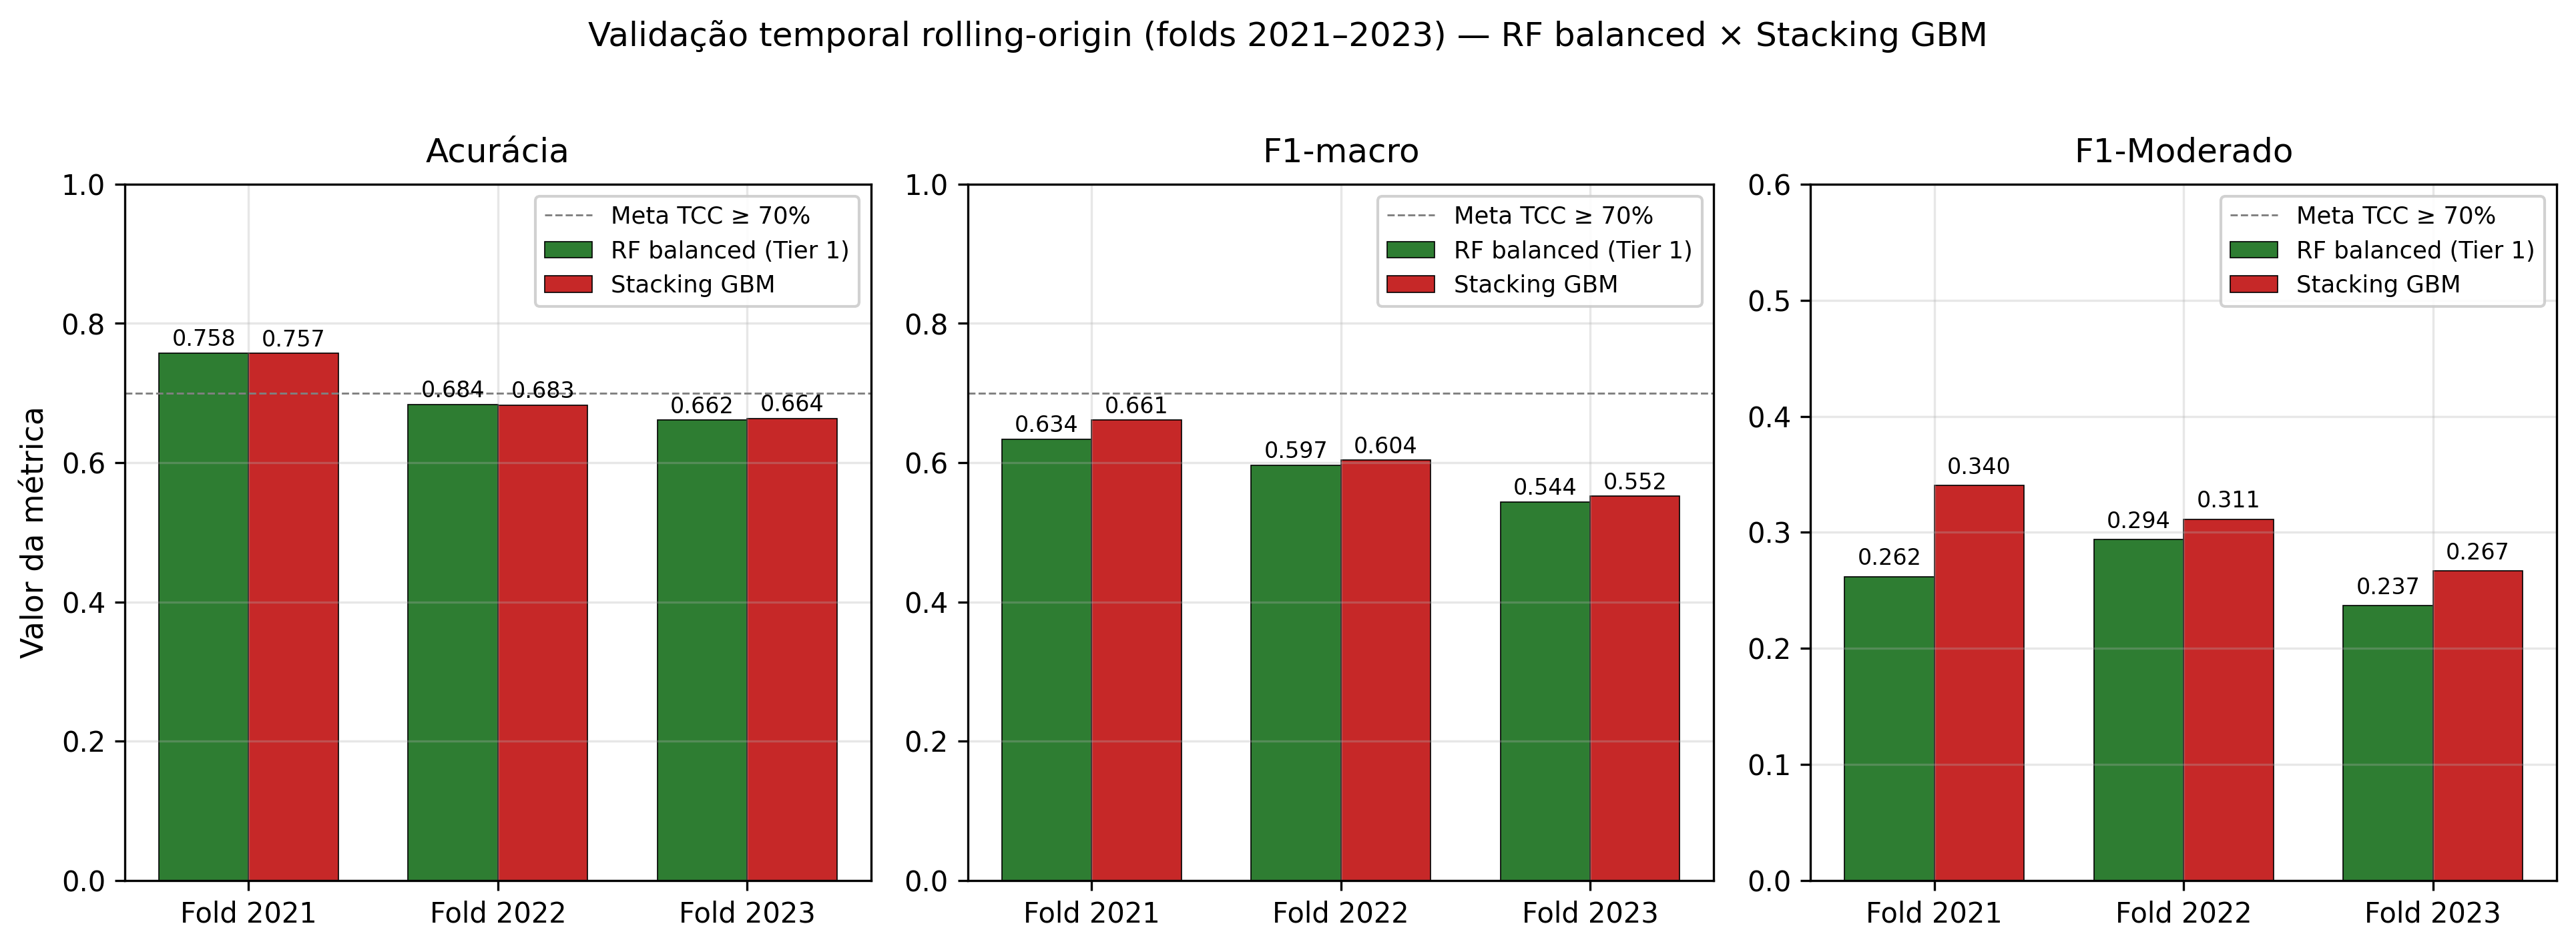
\includegraphics[width=\textwidth]{modelos/relatorios/validacao_temporal_comparativo.png}
\caption{Validação temporal \emph{rolling-origin} (\emph{folds} 2021--2023): RF balanceado Tier~1 \emph{vs.}\ \emph{Stacking} GBM em acurácia, $\text{F}_1$-macro e $\text{F}_1$-Moderado. Linha tracejada cinza indica a meta acadêmica original ($\geq \SI{70}{\percent}$).}
\label{fig:res_temporal_barras}
\end{figure}

A queda em \(\text{F}_1\)-Moderado sob validação temporal ($-$\SI{32,35}{pp} para o Stacking GBM) permanece o ponto frágil, motivando, como trabalho futuro \emph{prioritário}, a reimplementação das \emph{features} de janela móvel com \textbf{causalidade estrita} (computar \texttt{Precipitacao\_ma30} usando apenas dados \(\leq t\) do registro), conforme registrado no Capítulo~\ref{cap:conclusao}.

\paragraph{Por que reportar o \emph{split} aleatório como métrica principal?} O objetivo deste TCC é demonstrar a viabilidade do \emph{pipeline} em modo \emph{operacional} (mapa interativo: usuário consulta um ponto agora, recebe uma classe), não fazer previsão temporal estrita de calendário. Para o uso aplicado, o \emph{split} estratificado aleatório é a métrica que melhor reflete a precisão esperada no momento em que o usuário interage com o mapa. O \emph{rolling-origin} atua como \textbf{verificação cruzada honesta} que documenta a robustez do modelo sob condições de uso mais exigentes.

% ============================================================================
\section{Ajuste multi-classe de limiares de decisão}
\label{sec:res_threshold}

Conforme discutido na Seção~\ref{subsec:metod_thresholds}, a predição padrão dos classificadores probabilísticos usa \texttt{argmax}, regra que penaliza a classe intermediária \emph{Moderado}. O \emph{script} \texttt{scripts/ajustar\_threshold.py} varre uma grade de pares (\texttt{thr\_Moderado}, \texttt{thr\_Muito\_Alto}) \(\in \{0{,}30; 0{,}35; \ldots; 0{,}55\}^2\) (36~configurações), avaliando \(\text{F}_1\)-macro e \(\text{F}_1\)-Moderado em \num{50000} amostras estratificadas do conjunto de teste.

A Tabela~\ref{tab:res_threshold} mostra a configuração ótima para o modelo final. Tanto a otimização por \(\text{F}_1\)-macro quanto a por \(\text{F}_1\)-Moderado convergem para o mesmo ponto: \texttt{thr\_Moderado=0,35}, \texttt{thr\_Muito\_Alto=0,45}.

\begin{table}[h]
\centering
\caption{Resultado do \emph{threshold tuning} multi-classe (\texttt{ensemble\_stacking\_gbm}).}
\label{tab:res_threshold}
\begin{tabular}{lcccc}
\toprule
\textbf{Estratégia} & \textbf{Acurácia} & \textbf{$\text{F}_1$-macro} & \textbf{$\text{F}_1$-Moderado} & \textbf{$\Delta \text{F}_1$-Mod.} \\
\midrule
\emph{Baseline} (\texttt{argmax})    & 84,32\% & 0,7957 & 0,6231 & --- \\
$\text{F}_1$-macro / $\text{F}_1$-Mod. ótimo & 83,88\% & 0,7981 & \textbf{0,6375} & +1,44\,pp \\
\bottomrule
\end{tabular}
\end{table}

O ganho de \(\text{F}_1\)-Moderado (+\SI{1,44}{pp}) tem custo de \SI{0,44}{pp} em acurácia global --- \emph{trade-off} considerado favorável dada a relevância da classe intermediária. A configuração final é persistida em \texttt{modelos/prediction\_thresholds.json}.

% ============================================================================
\section{Evolução incremental do \emph{pipeline}}
\label{sec:res_evolucao}

A Tabela~\ref{tab:res_evolucao} sintetiza a evolução do desempenho ao longo das principais decisões metodológicas. A Figura~\ref{fig:res_evolucao} apresenta o mesmo dado de forma gráfica.

\begin{table}[h]
\centering
\caption{Evolução incremental do desempenho do \emph{pipeline}.}
\label{tab:res_evolucao}
\begin{tabular}{lccc}
\toprule
\textbf{Configuração} & \textbf{Acurácia} & \textbf{$\text{F}_1$-macro} & \textbf{$\text{F}_1$-Mod.} \\
\midrule
SGDClassifier (TCC II original)             & 62,43\% & 0,5864 & 0,3613 \\
\midrule
Ensemble Stacking (sem Tier 1)              & 80,49\% & 0,7492 & 0,5498 \\
\quad + 24 \emph{features} Tier 1           & 83,60\% & 0,7892 & 0,6168 \\
\quad + Optuna em XGBoost e LightGBM        & 84,14\% & 0,7944 & 0,6202 \\
\quad + meta-classificador GBM              & 84,61\% & 0,7995 & 0,6296 \\
\quad + \emph{thresholds} calibrados        & 83,88\% & 0,7981 & \textbf{0,6375} \\
\midrule
\textbf{$\Delta$ Stacking baseline $\to$ final} & \textbf{+3,39\,pp} & \textbf{+4,89\,pp} & \textbf{+8,77\,pp} \\
\textbf{$\Delta$ SGD $\to$ final}             & \textbf{+21,45\,pp} & \textbf{+21,17\,pp} & \textbf{+27,62\,pp} \\
\bottomrule
\end{tabular}
\end{table}

\begin{figure}[h]
\centering
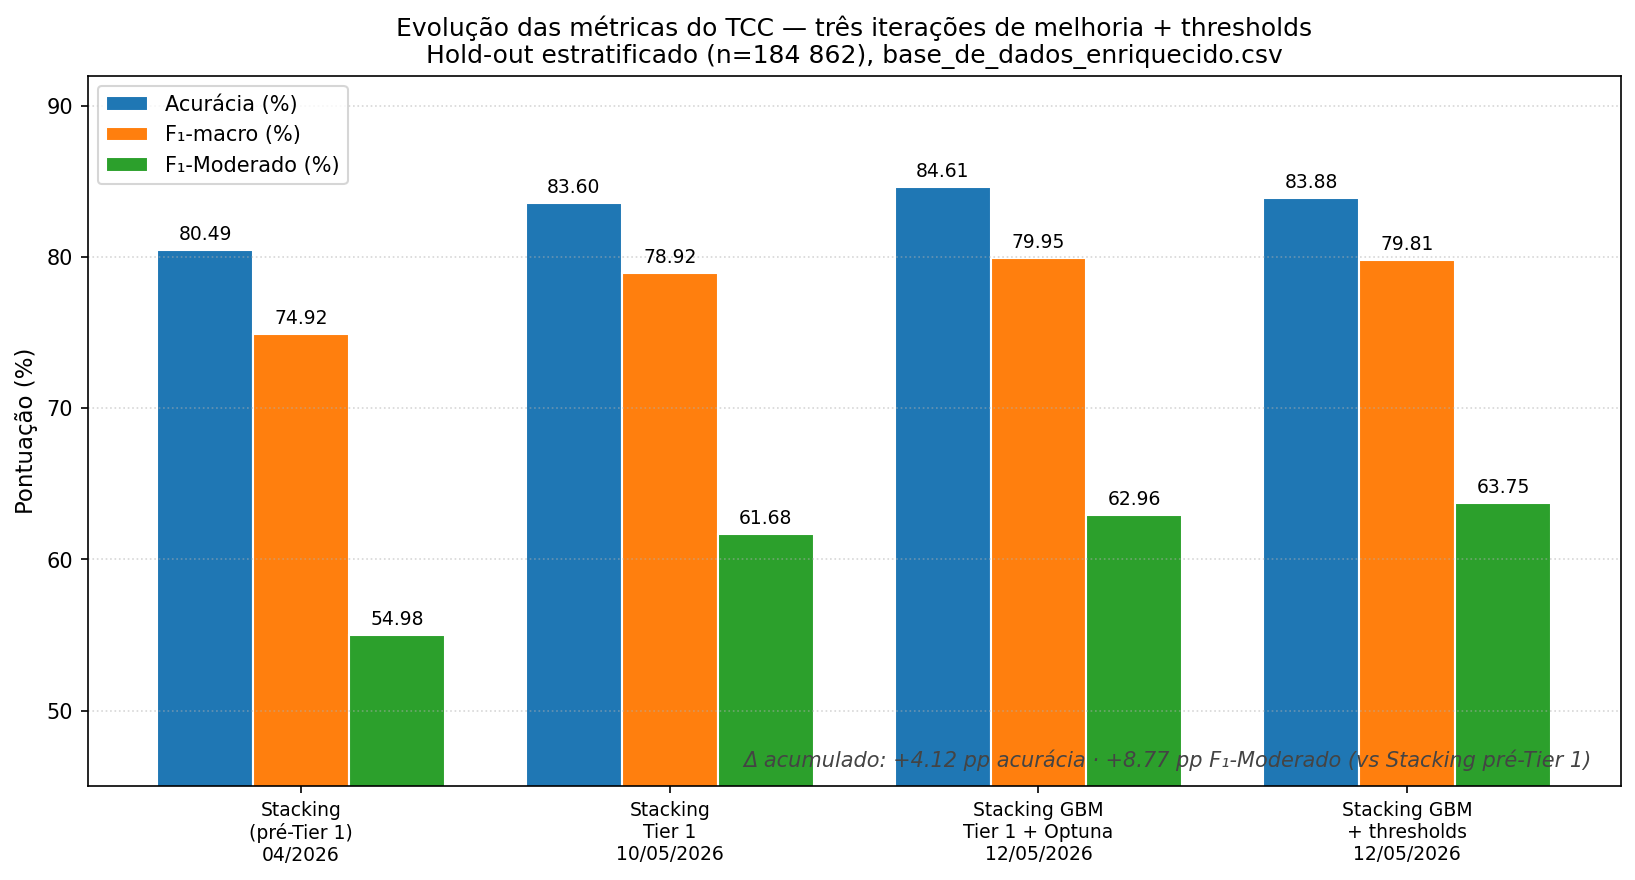
\includegraphics[width=0.85\textwidth]{modelos/relatorios/evolucao_modelos.png}
\caption{Evolução incremental da acurácia, $\text{F}_1$-macro e $\text{F}_1$-Moderado ao longo das principais decisões metodológicas.}
\label{fig:res_evolucao}
\end{figure}

Três marcos se destacam:

\begin{itemize}
  \item A \textbf{engenharia de \emph{features} físico-climáticas Tier 1} foi o fator dominante de ganho: +\SI{3,11}{pp} em acurácia e +\SI{6,70}{pp} em \(\text{F}_1\)-Moderado, ao custo de apenas 40~segundos de geração \emph{offline}. Esse resultado reforça a tese de que \emph{engenharia de variáveis bem embasada na literatura é tão importante quanto a escolha do algoritmo} em problemas de domínio.

  \item A \textbf{otimização bayesiana por Optuna} sobre XGBoost e LightGBM~\cite{akiba2019optuna} entregou +\SI{0,54}{pp} em acurácia como \emph{base learners} do \emph{stacking}.

  \item A substituição do meta-classificador de Logistic Regression por \textbf{Gradient Boosting}~\cite{friedman2001greedy} no \emph{stacking} produziu +\SI{0,47}{pp} em acurácia, +\SI{0,51}{pp} em \(\text{F}_1\)-macro e +\SI{0,94}{pp} em \(\text{F}_1\)-Moderado --- confirmando que arquiteturas de \emph{stacking} com meta-\emph{learner} mais expressivo se beneficiam de quantidade de dados suficiente, conforme antecipado por Wolpert~\cite{wolpert1992stacked}.
\end{itemize}

% ============================================================================
\section{Validação operacional via aplicação web}
\label{sec:res_app}

Para validar o \emph{pipeline} em modo \emph{operacional}, foram realizadas consultas comparativas no aplicativo web interativo descrito na Seção~\ref{sec:metod_app_web}. Dois pontos opostos da Amazônia Legal foram consultados em uma data de plena estação seca (setembro):

\begin{enumerate}
  \item Centro do estado do Amazonas (\(-3{,}5^\circ; -62{,}5^\circ\)): região historicamente úmida, baixa densidade de focos, vegetação intacta.
  \item Sul do estado do Pará (\(-8{,}5^\circ; -50{,}5^\circ\)): região de arco do desmatamento, alta densidade histórica de focos.
\end{enumerate}

A Tabela~\ref{tab:res_smoke} apresenta os resultados.

\begin{table}[h]
\centering
\caption{Consultas comparativas no aplicativo web (\texttt{ensemble\_stacking\_gbm}, mês = setembro).}
\label{tab:res_smoke}
\small
\begin{tabular}{lcccc}
\toprule
\textbf{Ponto consultado} & \textbf{Risco previsto} & \textbf{Confiança} & \textbf{SPI-1m} & \textbf{KBDI \emph{proxy}} \\
\midrule
Centro AM ($-3{,}5; -62{,}5$) & Baixo       & 82,3\% & $0{,}00$ & $2{,}4$ \\
Sul PA ($-8{,}5; -50{,}5$)    & \textbf{Muito Alto} & \textbf{92,9\%} & $-0{,}57$ & $\mathbf{418{,}6}$ \\
\bottomrule
\end{tabular}
\end{table}

O modelo discrimina corretamente os dois cenários, com explicações fisicamente defensáveis emitidas pelo \emph{explainer}: para o ponto AM, as variáveis dominantes a favor da classe \emph{Baixo} são \texttt{DiaSemChuva} (\(\downarrow\)), \texttt{Indice\_Seca} (\(\downarrow\)) e \texttt{Dias\_Desde\_Ultimo\_Incêndio} (\(\uparrow\)); para o ponto PA, as variáveis dominantes a favor da classe \emph{Muito Alto} são \texttt{DiaSemChuva} (\(\downarrow\) período de estiagem), \texttt{Indice\_Seca} (\(\uparrow\)), \texttt{SPI-1m} (\(\uparrow\) déficit), \texttt{SPI-3m} (\(\uparrow\) déficit prolongado) e \texttt{Temp\_Climatologica} (\(\uparrow\)). O tempo médio de resposta da API \texttt{/api/predict} para ambos os pontos foi de \(11\) a \SI{18}{\second}, dominado pela latência das chamadas externas (NASA POWER + NASA FIRMS), aceitável para o uso interativo.

A aplicação está documentada em \texttt{README\_APP.md} e o código-fonte está disponível em \texttt{scripts/app\_map\_interativo.py}. A interface foi testada nas resoluções $1280 \times 720$ (\emph{notebook} típico) e $1920 \times 1080$ (\emph{desktop}), com painel lateral fixo de \num{420}\,px e mapa centralizado responsivo (Leaflet 1.9.4~\cite{leafletjs} sob Folium 0.16~\cite{folium}).
